\documentclass[12pt,a4paper]{article}

% 导入必要的宏包
\usepackage[UTF8]{ctex}
\usepackage{geometry}
\usepackage{amsmath}
\usepackage{amsfonts}
\usepackage{amssymb}
\usepackage{graphicx}
\usepackage{enumitem}
\usepackage{xcolor}
\usepackage{tikz}
\usepackage{float}
\usepackage{hyperref}
\usepackage{multicol}
\usepackage{longtable}
\usepackage{array}
\usepackage{tabularx}

% 页面设置
\geometry{left=2.5cm,right=2.5cm,top=2.5cm,bottom=2.5cm}

% 标题页设置
\title{\textbf{2009年数据结构题库} \\ \large }
\author{}
\date{}

% 定义题型环境
\newenvironment{choicequestion}[1][]{%
    \vspace{0.5cm}
    \noindent\textbf{[#1]}
    \vspace{0.2cm}
}{}

\newenvironment{answersection}{%
    \vspace{0.2cm}
    \noindent\textbf{[参考答案]}\\
    \vspace{0.1cm}
}{}

\newenvironment{analysissection}{%
    \vspace{0.2cm}
    \noindent\textbf{[答案解析]}\\
    \vspace{0.1cm}
}{}

% 定义题号计数器
\newcounter{questioncounter}

% 问题格式化命令
\newcommand{\question}[2]{%
    \stepcounter{questioncounter}%
    \noindent\textbf{\thequestioncounter} #1%
    % \begin{flushright}
    %     （  ）
    % \end{flushright}
}

% 选择题选项格式
\newcommand{\choices}[4]{%
    \begin{multicols}
    \noindent \textbf{A.} #1 \par
    \noindent \textbf{B.} #2 \par
    \noindent \textbf{C.} #3 \par
    \noindent \textbf{D.} #4 \par
    \end{multicols}%
}

% 表格格式
\newcolumntype{Y}{>{\centering\arraybackslash}X}

% 开始文档
\begin{document}

\maketitle

\section{单项选择题}

\begin{choicequestion}[单选题]
\question{为解决计算机主机与打印机之间速度不匹配问题，通常设置一个打印数据缓冲区，主机将要输出的数据依次写入该缓冲区，而打印机则依次从该缓冲区中取出数据。该缓冲区的逻辑结构应该是}{B}
\choices{栈}{队列}{树}{图}

\begin{answersection}
B. 队列
\end{answersection}

\begin{analysissection}
这是一个典型的队列应用场景。主机将要打印的数据依次写入缓冲区，打印机依次从缓冲区中取出数据，这是先进先出（FIFO）的操作模式，符合队列的特性。
\end{analysissection}
\end{choicequestion}

\begin{choicequestion}[单选题]
\question{设栈 S 和队列 Q 的初始状态均为空，元素 a, b, c, d, e, f, g 依次进入栈 S。若每个元素出栈后立即进入队列 Q，且 7 个元素出队的顺序是 b, d, c, f, e, a, g，则栈 S 的容量至少是}{C}
\choices{1}{2}{3}{4}

\begin{answersection}
C. 3
\end{answersection}

\begin{analysissection}
要确定栈的容量，我们需要模拟元素进出的过程。按题目要求，要得到出队序列 b, d, c, f, e, a, g，我们可以分析：
1. a, b入栈，b出栈并入队
2. c入栈，d入栈，d出栈并入队
3. c出栈并入队
4. e, f入栈，f出栈并入队
5. e出栈并入队
6. a出栈并入队
7. g入栈，g出栈并入队

在这个过程中，栈中最多同时存在3个元素（例如在第4步之前，栈中有a, e, f），所以栈的容量至少是3。
\end{analysissection}
\end{choicequestion}

\begin{choicequestion}[单选题]
\question{给定二叉树如右图所示。设 N 代表二叉树的根，L 代表根结点的左子树，R 代表根结点的右子树。若遍历后的结点序列是 $3,1,7,5,6,2,4$ ，则其遍历方式是}{D}

\begin{figure}[H]
\centering
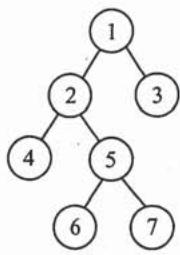
\includegraphics[width=0.3\textwidth]{images/74b452b20028944e66ef9c9fdd4ce103cb68a6453d068853d52f531b54f685e8.jpg}
\end{figure}

\choices{LRN}{NRL}{RLN}{RNL}

\begin{answersection}
D. RNL
\end{answersection}

\begin{analysissection}
根据遍历序列3,1,7,5,6,2,4，我们可以分析遍历顺序：先访问右子树（R），再访问根节点（N），最后访问左子树（L），这就是RNL遍历方式。
\end{analysissection}
\end{choicequestion}

\begin{choicequestion}[单选题]
\question{下列二叉排序树中，满足平衡二叉树定义的是}{}

\begin{multicols}{2}
\begin{enumerate}[label=(\Alph*)]
    \item 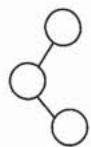
\includegraphics[width=0.4\textwidth]{images/4f31d5994e2861a28ce02d5cdfbd8f4e56b73dbd6861caf0ef11017b2ff1ae00.jpg}
    \item 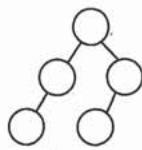
\includegraphics[width=0.4\textwidth]{images/f3ba9af2f98c94f3d6bc5aa142f11778d30b2bba0f85047a8a2444832ae17f50.jpg}
    \item 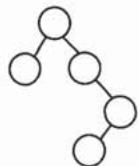
\includegraphics[width=0.4\textwidth]{images/e45f456ec26be3cd5ced6a89407f1aff0b9f3bc7d2c5b115b77ccbdfc92bbdcb.jpg}
    \item 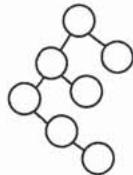
\includegraphics[width=0.4\textwidth]{images/71eb835cebd2633945806a3884deecbe6dd1a0306e2291bb20689a833f28cc2d.jpg}
\end{enumerate}
\end{multicols}

\begin{answersection}
根据图像判断平衡二叉树（左右子树高度差不超过1）
\end{answersection}

\begin{analysissection}
平衡二叉树是指对于任何一个节点，它的左右子树的高度差不超过1。需要逐个检查各选项中的树是否满足这一条件。
\end{analysissection}
\end{choicequestion}

\begin{choicequestion}[单选题]
\question{已知一棵完全二叉树的第 6 层（设根为第 1 层）有 8 个叶结点，则该完全二叉树的结点个数最多是}{D}
\choices{39}{52}{111}{119}

\begin{answersection}
D. 119
\end{answersection}

\begin{analysissection}
在完全二叉树中，如果某一层有叶结点，这些叶结点一定在最右边。
设第6层有x个非叶结点，8个叶结点。
第5层有16个结点，设前a个结点各有2个子结点，后(16-a)个结点各有1个子结点。
则a+b=16，其中b=16-a表示第5层后b个结点各有1个子结点。
第6层有2a+b个结点，其中b个是叶结点。
由题意知b=8，所以a=8。
第6层有2a+b=16+8=24个结点，其中16个非叶结点，8个叶结点。
第7层最多有2a=16个结点。
前5层：31个
第6层：24个
第7层：16个
总共：31+24+16=71个（这只是最小值）

但题目要求最大值，所以我们考虑第6层满的情况：
第6层有32个结点，其中28个非叶结点，4个叶结点。
第7层最多有28×2=56个结点。
总数=31+32+56=119个。

所以答案是D. 119。
\end{analysissection}
\end{choicequestion}

\begin{choicequestion}[单选题]
\question{将森林转换为对应的二叉树，若在二叉树中，结点 $\mathbf{u}$ 是结点 $\mathbf{v}$ 的父结点的父结点，则在原来的森林中， $\mathbf{u}$ 和 $\mathbf{v}$ 可能具有的关系是}{}
\begin{enumerate}
    \item 父子关系
    \item 兄弟关系
    \item u的父结点与 $\mathbf{v}$ 的父结点是兄弟关系
\end{enumerate}

\choices{只有 II}{I 和 II}{I 和 III}{I、II 和 III}

\begin{answersection}
B. I 和 II
\end{answersection}

\begin{analysissection}
在森林转换为二叉树的过程中，使用"左孩子右兄弟"表示法：
- 左子结点关系表示父子关系
- 右子结点关系表示兄弟关系

在二叉树中u是v的祖父结点，可能对应森林中的情况：
1. u和v是父子关系（可能u是v的父亲的父亲）
2. u和v是兄弟关系（可能u是v的父节点的兄弟）

情况III不太可能出现，因为u是v的祖父，这意味着他们在树的同一路径上，不太可能满足情况III的关系。
\end{analysissection}
\end{choicequestion}

\section{综合应用题}

\begin{choicequestion}[问答题]
\question{带权图（权值非负，表示边连接的两顶点间的距离）的最短路径问题是找出从初始顶点到目标顶点之间的一条最短路径。假设从初始顶点到目标顶点之间存在路径，现有一种解决该问题的方法：\newline
(1) 设最短路径初始时仅包含初始顶点, 令当前顶点 $\mathbf{u}$ 为初始顶点;  \newline
(2) 选择离 $\mathbf{u}$ 最近且尚未在最短路径中的一个顶点 $\mathbf{v}$ , 加入最短路径中, 修改当前顶点 $\mathbf{u} = \mathbf{v}$ ;  \newline
(3) 重复步骤(2), 直到 u 是目标顶点时为止。  \newline
请问上述方法能否求得最短路径？若该方法可行，请证明之；否则，请举例说明。}{}

\begin{answersection}
该方法不可行，不能保证求得最短路径。
\end{answersection}

\begin{analysissection}
该方法实际上是贪心策略，每次选择当前最近的顶点，但这不能保证最终路径最短。

反例：
设有4个顶点A(起始)、B、C、D(目标)，边及权重如下：
- A-B: 2
- A-C: 3
- B-D: 100
- C-D: 4

按该算法：
1. 路径={A}, u=A
2. 选择离A最近的顶点B，路径={A,B}, u=B
3. 选择离B最近且不在路径中的顶点，只有D（C已被跳过），路径={A,B,D}

路径A→B→D的总权重为2+100=102。

但最短路径是A→C→D，总权重为3+4=7。

因此，该方法不能求得最短路径。
\end{analysissection}
\end{choicequestion}

\begin{choicequestion}[问答题]
\question{已知一个带有表头结点的单链表，结点结构为\newline
\begin{table}[h]
\centering
\begin{tabular}{|c|c|}
\hline
data & link \\
\hline
\end{tabular}
\end{table}
\newline
假设该链表只给出了头指针 list。在不改变链表的前提下，请设计一个尽可能高效的算法，查找链表中倒数第 $k$ 个位置上的结点（ $k$ 为正整数）。若查找成功，算法输出该结点的 data 域的值，并返回 1；否则，只返回 0。要求：\newline
1）描述算法的基本设计思想。\newline
2）描述算法的详细实现步骤。\newline
3）根据设计思想和实现步骤，采用程序设计语言描述算法（使用 C、C++ 或 Java 语言实现），关键之处请给出简要注释。}{}

\begin{answersection}
算法实现如下：
\end{answersection}

\begin{analysissection}
1）算法基本设计思想：
使用双指针技术（快慢指针）。设置两个指针p和q，初始都指向头结点。先让p向前移动k步，然后p和q同时向前移动，直到p到达链表末尾。此时q指向的就是倒数第k个结点。

2）算法详细实现步骤：
- 初始化两个指针p和q，都指向头结点
- 让p向前移动k步
- 如果p已经到达链表末尾，说明k大于链表长度，返回0
- 同时移动p和q，直到p到达链表末尾
- 此时q指向倒数第k个结点
- 输出data域值并返回1

3）C语言实现：
\end{analysissection}
\end{choicequestion}

\end{document}